\documentclass[11pt]{beamer}%
\usepackage{graphicx, amssymb, amsmath, color, verbatim,tikz, hyperref, complexity,mathtools, etoolbox, dsfont, verbatim, stackrel, stmaryrd}
\usetheme{Singapore}
%\usecolortheme{seagull}
\usepackage{libertine}
\usepackage[T1]{fontenc}
\usepackage{tikz}
\usetikzlibrary{arrows,positioning,shadows,shadings}

\definecolor{darkred}{rgb}{0.6,.1,.1}
\definecolor{darkblue}{rgb}{.1,.1,0.5}
\definecolor{darkgreen}{rgb}{.1,.3,.1}
\newcommand{\red}{\color{darkred}}
\newcommand{\blue}{\color{darkblue}}
\newcommand{\green}{\color{darkgreen}}
\renewcommand{\bigskip}{\medskip\medskip\medskip}
\newcommand{\auth}[1]{{\green\hfill{\footnotesize #1}}}
\newtheorem{observation}{Observation}
\newcommand{\calG}{\mathcal{G}}
\newcommand{\td}{\mathit{td}}
\newcommand{\tw}{\mathit{tw}}
\newcommand{\pw}{\mathit{pw}}
\newcommand{\mecp}{\mathrm{MECP}}
\renewcommand{\em }{\red}
\newcommand{\RR}{\mathbb{R}}

\newcommand{\eqdef}{\mbox{\,\raisebox{0.2ex}{\scriptsize\ensuremath{\mathrm:}}\ensuremath{=}\,}} % \
\renewcommand{\b}[1]{{\boldsymbol{#1}}} % bold letters

% Loday and anti-Loday accents (?)
\makeatletter
\newcommand{\oset}[3][0ex]{%
  \mathrel{\mathop{#3}\limits^{
    \vbox to#1{\kern-2\ex@
    \hbox{$\scriptstyle#2$}\vss}}}}
%
\newcommand{\uset}[3][0ex]{%
  \mathrel{\mathop{#3}\limits_{
    \vbox to#1{\kern-7\ex@
    \hbox{$\scriptstyle#2$}\vss}}}}
\makeatother
%
\newcommand{\loday}[1]{\smash{\overset{\frown}{#1}}}
\newcommand{\antiloday}[1]{\smash{\overset{\smile}{#1}}}
\newcommand{\upArc}[1]{\smash{\raisebox{.05cm}{$\uset[0ex]{#1}{\frown}$}}}
\newcommand{\downArc}[1]{\smash{\raisebox{-.05cm}{$\oset[.2ex]{#1}{\smile}$}}}
% yin and yang accents (?)
\newcommand{\yin}[1]{\smash{\overset{\sim}{#1}}}
\newcommand{\yang}[1]{\smash{\overset{\backsim}{#1}}}
\newcommand{\yinArc}[2]{\smash{\raisebox{.05cm}{$\uset[0ex]{#1}{\frown}$}\hspace{-.3ex}\raisebox{-.03cm}{$\oset[.2ex]{#2}{\smile}$}}}
\newcommand{\yangArc}[2]{\smash{\raisebox{-.03cm}{$\oset[.2ex]{#1}{\smile}$}\hspace{-.3ex}\raisebox{.05cm}{$\uset[0ex]{#2}{\frown}$}}}
% weak and strong equivalence on S_n
\newcommand{\weakeq}{\asymp}
\newcommand{\strongeq}{\mathbin{\smash{\begin{smallmatrix} \backsim \\[-.3cm] \sim \end{smallmatrix}}}}% % J: I would like to stack \backsim and \sim instead

\setbeamertemplate{navigation symbols}{}%remove navigation symbols
\setbeamertemplate{footline}[frame number]

\title{Combinatorics of Rectangulations}

  \author{{\em  Jean Cardinal}\\
    Universit\'e libre de Bruxelles (ULB)}
  
  \date{Jagiellonian TCS Seminar -- April 2024}

\begin{document}

%--------------
%--- title page
%--------------
{
\frame{\titlepage}
}

%----------------
%--- Introduction
%----------------

\begin{frame}
  \frametitle{Collaborators}
  \begin{tabular}{cccc}
    Andrei Asinowski & Stefan Felsner & \'Eric Fusy &  Vincent Pilaud \\
    \end{tabular}
  \begin{center}
  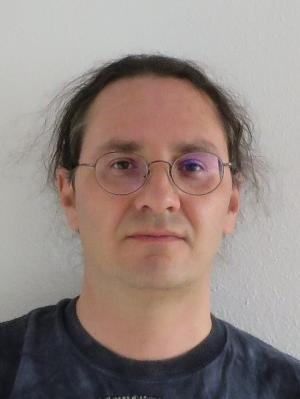
\includegraphics[height=.3\textheight]{asinowski.jpg}\ \ \ 
  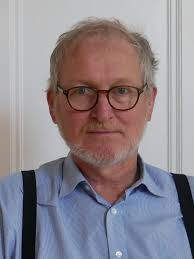
\includegraphics[height=.3\textheight]{felsner.jpg}\ \ \ 
  
\includegraphics[height=.3\textheight]{fusy.jpeg}\ \ \ 
  
\includegraphics[height=.3\textheight]{pilaud.jpg}
  \end{center}
  \begin{description}
  \item[Order \& Geometry 2022.] September 13-18, 2022, Ciążeń, Poland
    \item[] Stefan Felsner and Piotrek Micek
    \item[Combinatorics, Algorithms, and Geometry.] March 4-8, 2024, Dresden, Germany
    \item[] Namrata and Torsten M\"utze      
  \end{description}

\end{frame}

\begin{frame}
  \frametitle{Rectangulations and Combinatorics}
  \begin{center}
  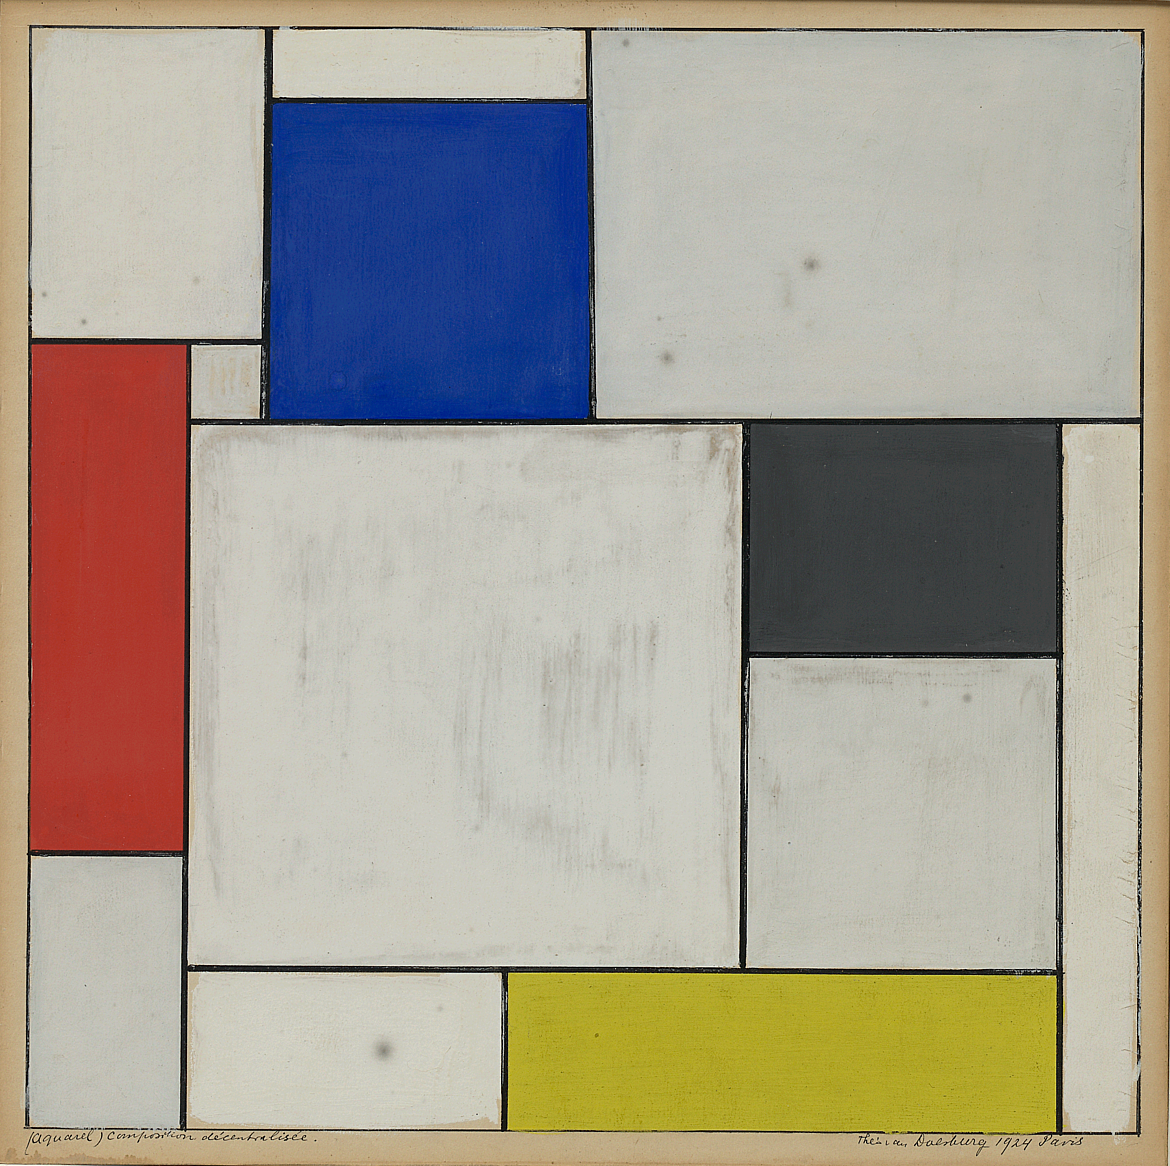
\includegraphics[height=.6\textheight]{doesburg.png}
  \end{center}
  \begin{description}
  \item[Bijective] Permutation classes
  \item[Order-theoretic] Lattice congruences
  \item[Polyhedral] Generalized permutahedra
  \end{description}  
\end{frame}

\begin{frame}
  \frametitle{Permutations}
  \begin{description}
  \item[Order-theoretic] Weak order
  \item[Polyhedral] Permutahedron
  \end{description}
    \begin{center}
      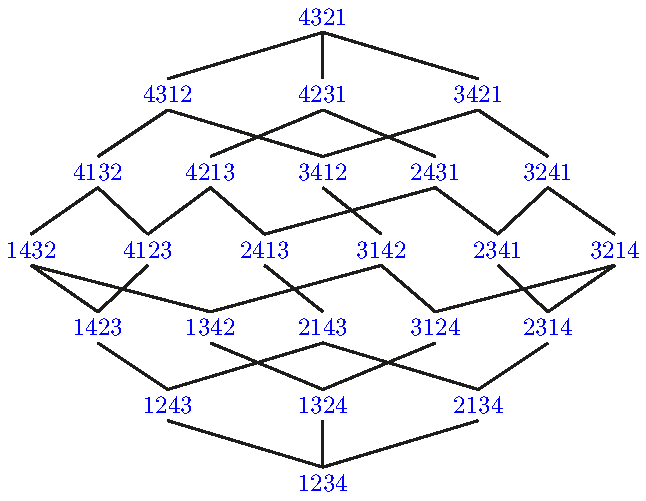
\includegraphics[height=.5\textheight]{weakOrderLeft4.pdf}
      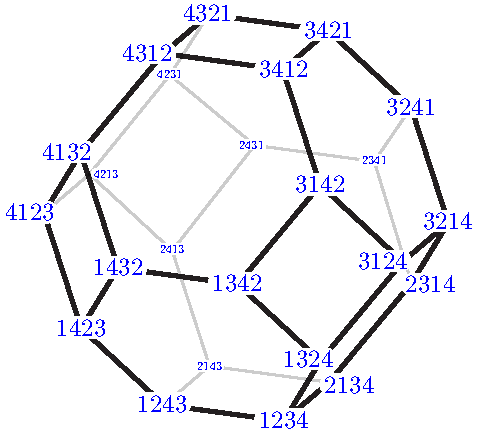
\includegraphics[height=.5\textheight]{permutahedronLeft4.pdf}
    \end{center}
\end{frame}

%---------------------------------
%--- Catalan, Tamari, Associahedra
%---------------------------------

\begin{frame}
  \frametitle{Binary trees}
  \begin{center}
      \includegraphics[page=4,height=.2\textheight]{figures.pdf} 
      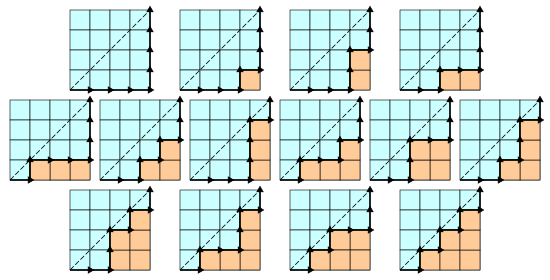
\includegraphics[height=.2\textheight]{catalan1.png}\ \  
      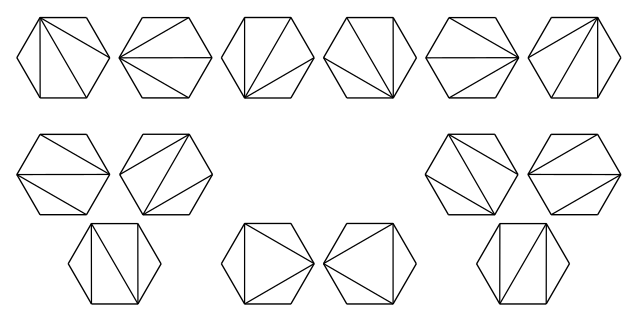
\includegraphics[height=.2\textheight]{catalan2.png}
    \end{center}
\auth{\scriptsize{(Wikimedia commons)}}
  \begin{description}
  \item[Bijective] Catalan families
  \item[Order-theoretic] Tamari lattice
  \item[Polyhedral] Associahedra
  \end{description}
\end{frame}

\begin{frame}
  \frametitle{Tamari lattice}
  Linear extensions of binary tree posets.
  \begin{center}
    \includegraphics[page=5, height=.2\textheight]{figures.pdf}
  \end{center}
  \pause
  
  \begin{center}
    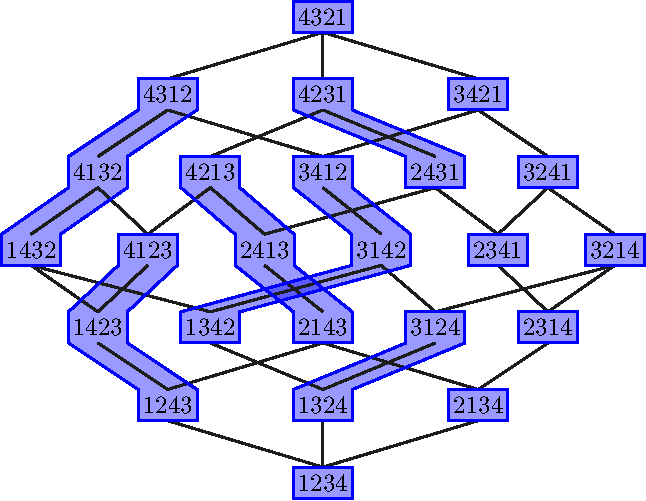
\includegraphics[height=.55\textheight]{weakOrderCongruence4.pdf}
    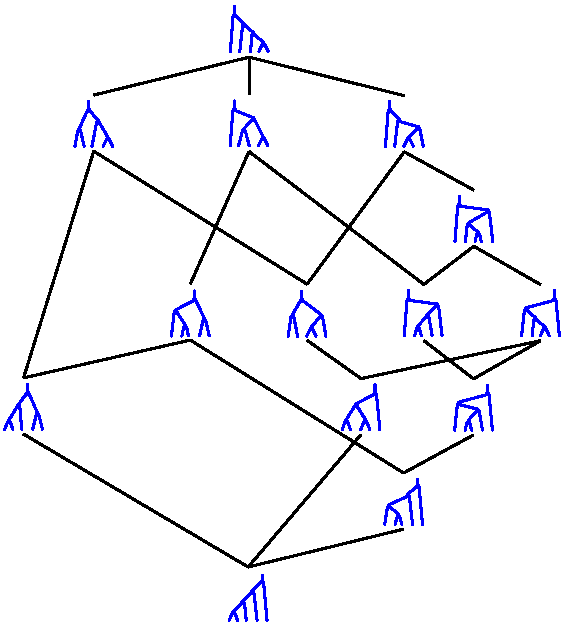
\includegraphics[height=.55\textheight]{TamariLattice4.pdf}
  \end{center}
  \auth{Tamari 1951}
\end{frame}

\begin{frame}
  \frametitle{The sylvester congruence}
    \begin{center}
      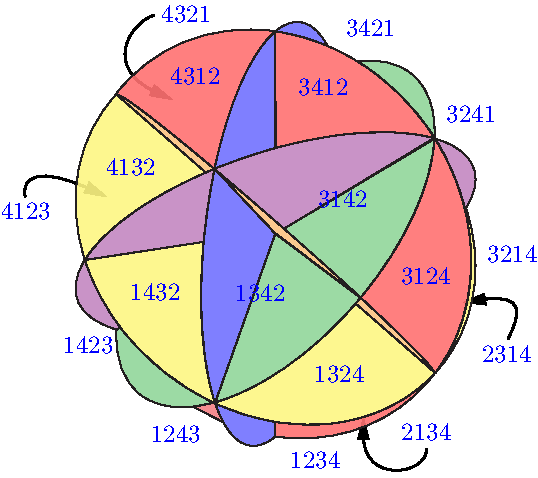
\includegraphics[height=.5\textheight]{braidFanLeft4.pdf}
      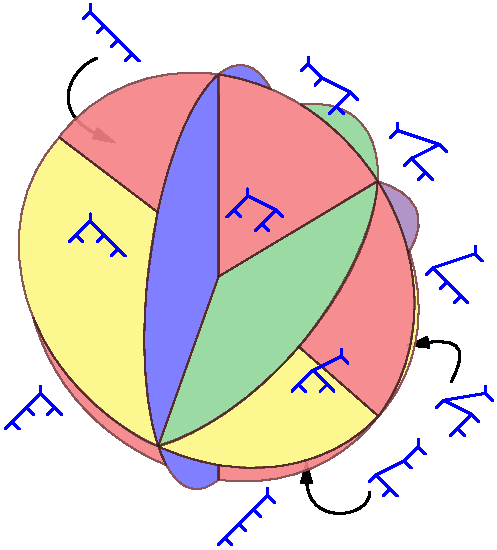
\includegraphics[height=.5\textheight]{sylvesterFan4.pdf}
    \end{center}
\end{frame}

\begin{frame}
  \frametitle{Lattice congruences}
  An equivalence relation $\equiv$ is a {\em lattice congruence} if it respects joins and meets:
  $$
  (x\equiv x' \mathrm{and\ } y\equiv y')\implies (x\vee y\equiv x'\vee y'\mathrm{and\ }  x\wedge y\equiv x'\wedge y') 
  $$
  \pause
  \begin{theorem}
    For any congruence of the weak order, gluing together the cones of the braid fan corresponding to the same congruence class yields the normal fan of a polytope.
  \end{theorem}
  % statement
  \auth{Pilaud-Santos~2019}

  \pause
  The cover graph of the {\em lattice quotient} is the skeleton of the polytope, called a {\em quotientope}.
\end{frame}

\begin{frame}
  \frametitle{Associahedra}
    \begin{center}
      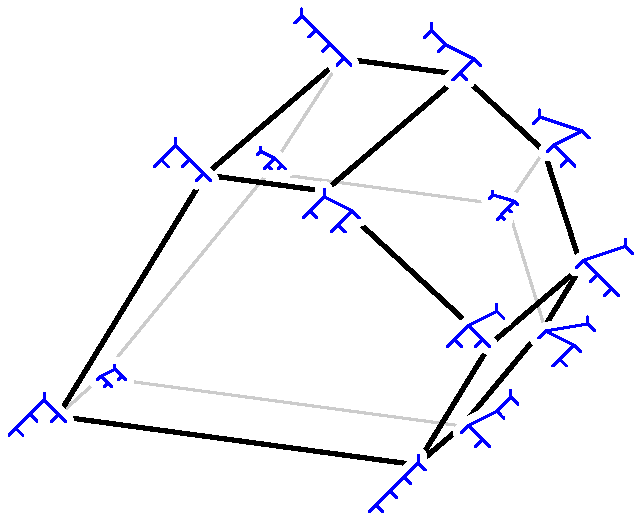
\includegraphics[height=.7\textheight]{associahedron4.pdf}
    \end{center}
    \auth{Stasheff 1963}
\end{frame}

\begin{frame}
  \frametitle{Loday coordinates}

  \begin{theorem}
  The associahedron is realized by the convex hull of the points
  \[
  \sum_{i\in [n]} \ell^T_i\cdot r^T_i \cdot \b{e}_i
  \]
  for all binary trees~$T$ with $n$ internal nodes, where $\ell^T_i$ and $r^T_i$ denote the number of leaves in the left and right subtrees of $i$ in $T$.
  \end{theorem}
  \auth{Loday 2004}  
\end{frame}

%------------------------
%--- Weak rectangulations
%------------------------

\begin{frame}
  \frametitle{Diagonal rectangulations and twin binary trees}
  \begin{center}
    \includegraphics[page=3, width=.8\textwidth]{figures.pdf}
  \end{center}
  Gluing two ``twin'' binary trees yields a {\em diagonal rectangulation}.
\end{frame}

\begin{frame}
  \frametitle{Weak rectangulations}
  Weak equivalence relation:
    \begin{center}
      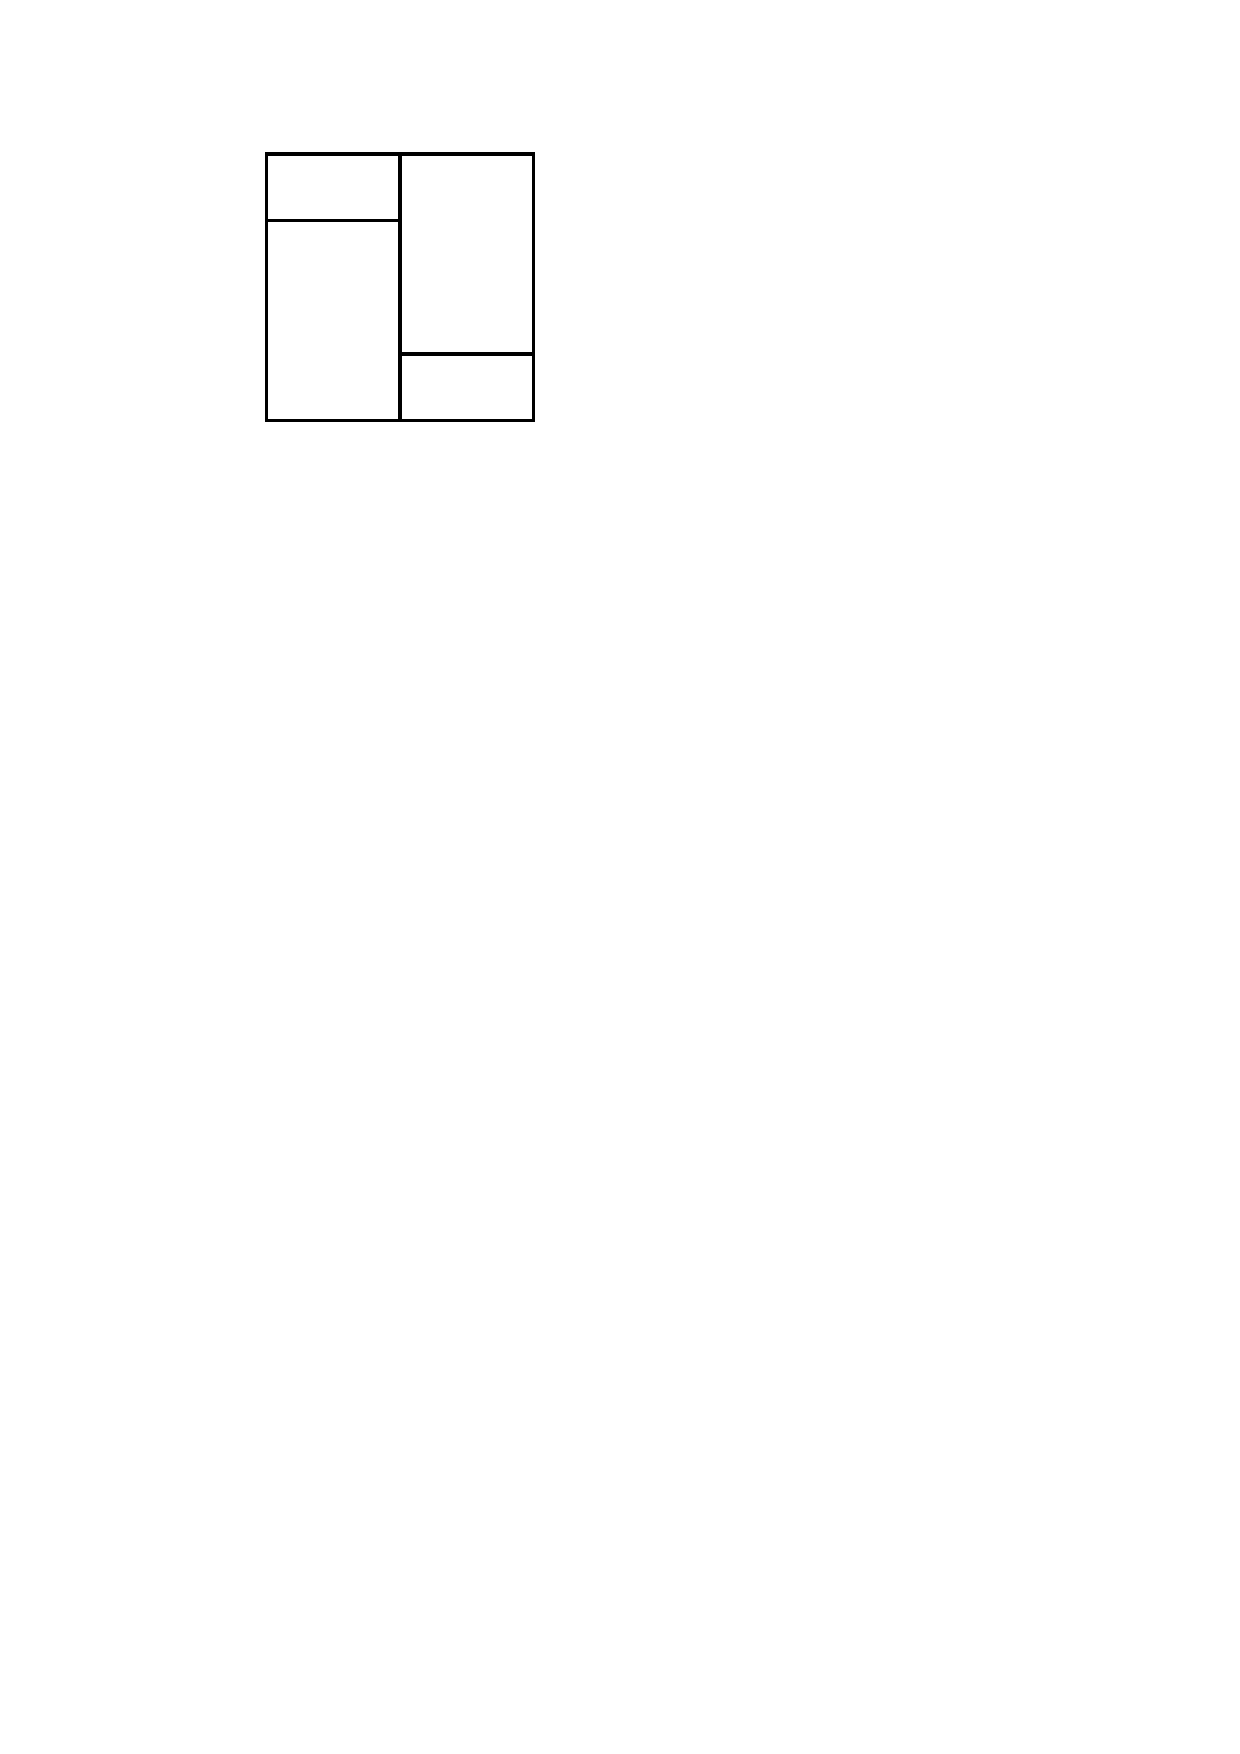
\includegraphics[page=1,height=.1\textheight]{figures.pdf} $\equiv$ 
      \includegraphics[page=2,height=.1\textheight]{figures.pdf}
    \end{center}   
    \begin{center}
      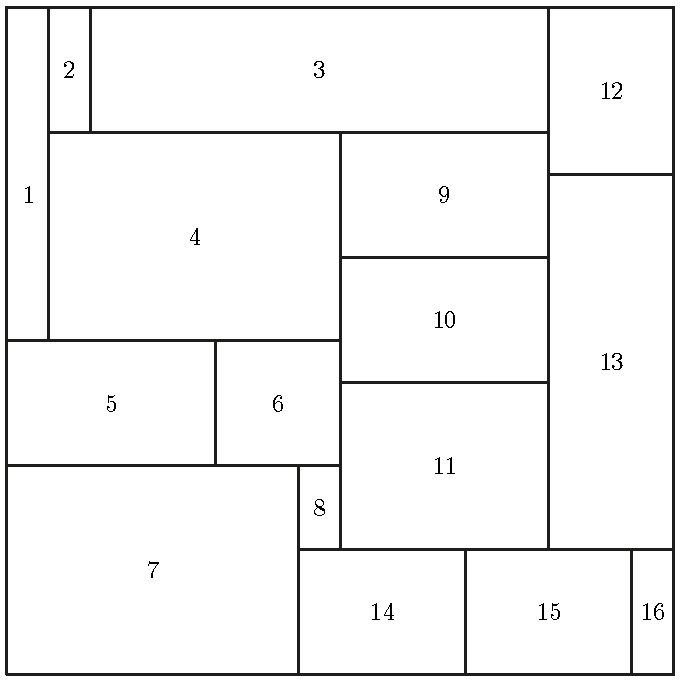
\includegraphics[height=.4\textheight]{strongRectangulation.pdf} $\equiv$ 
      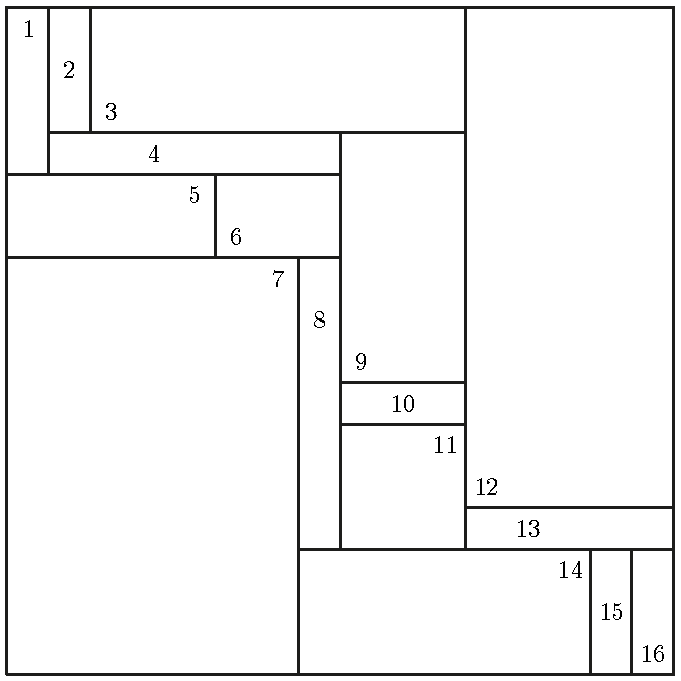
\includegraphics[height=.4\textheight]{weakRectangulation.pdf}
    \end{center}  
  \pause
  \begin{description}
  \item[Bijective] {\em Baxter} permutations, avoiding 2{\green 41}3 and 3{\green 14}2
    \pause
  \item[Order-theoretic] Weak rectangulation congruence
  \item[Polyhedral] Weak rectangulotopes
  \end{description}
\end{frame}

\begin{frame}
  \frametitle{Adjacency poset}
    \begin{center}
      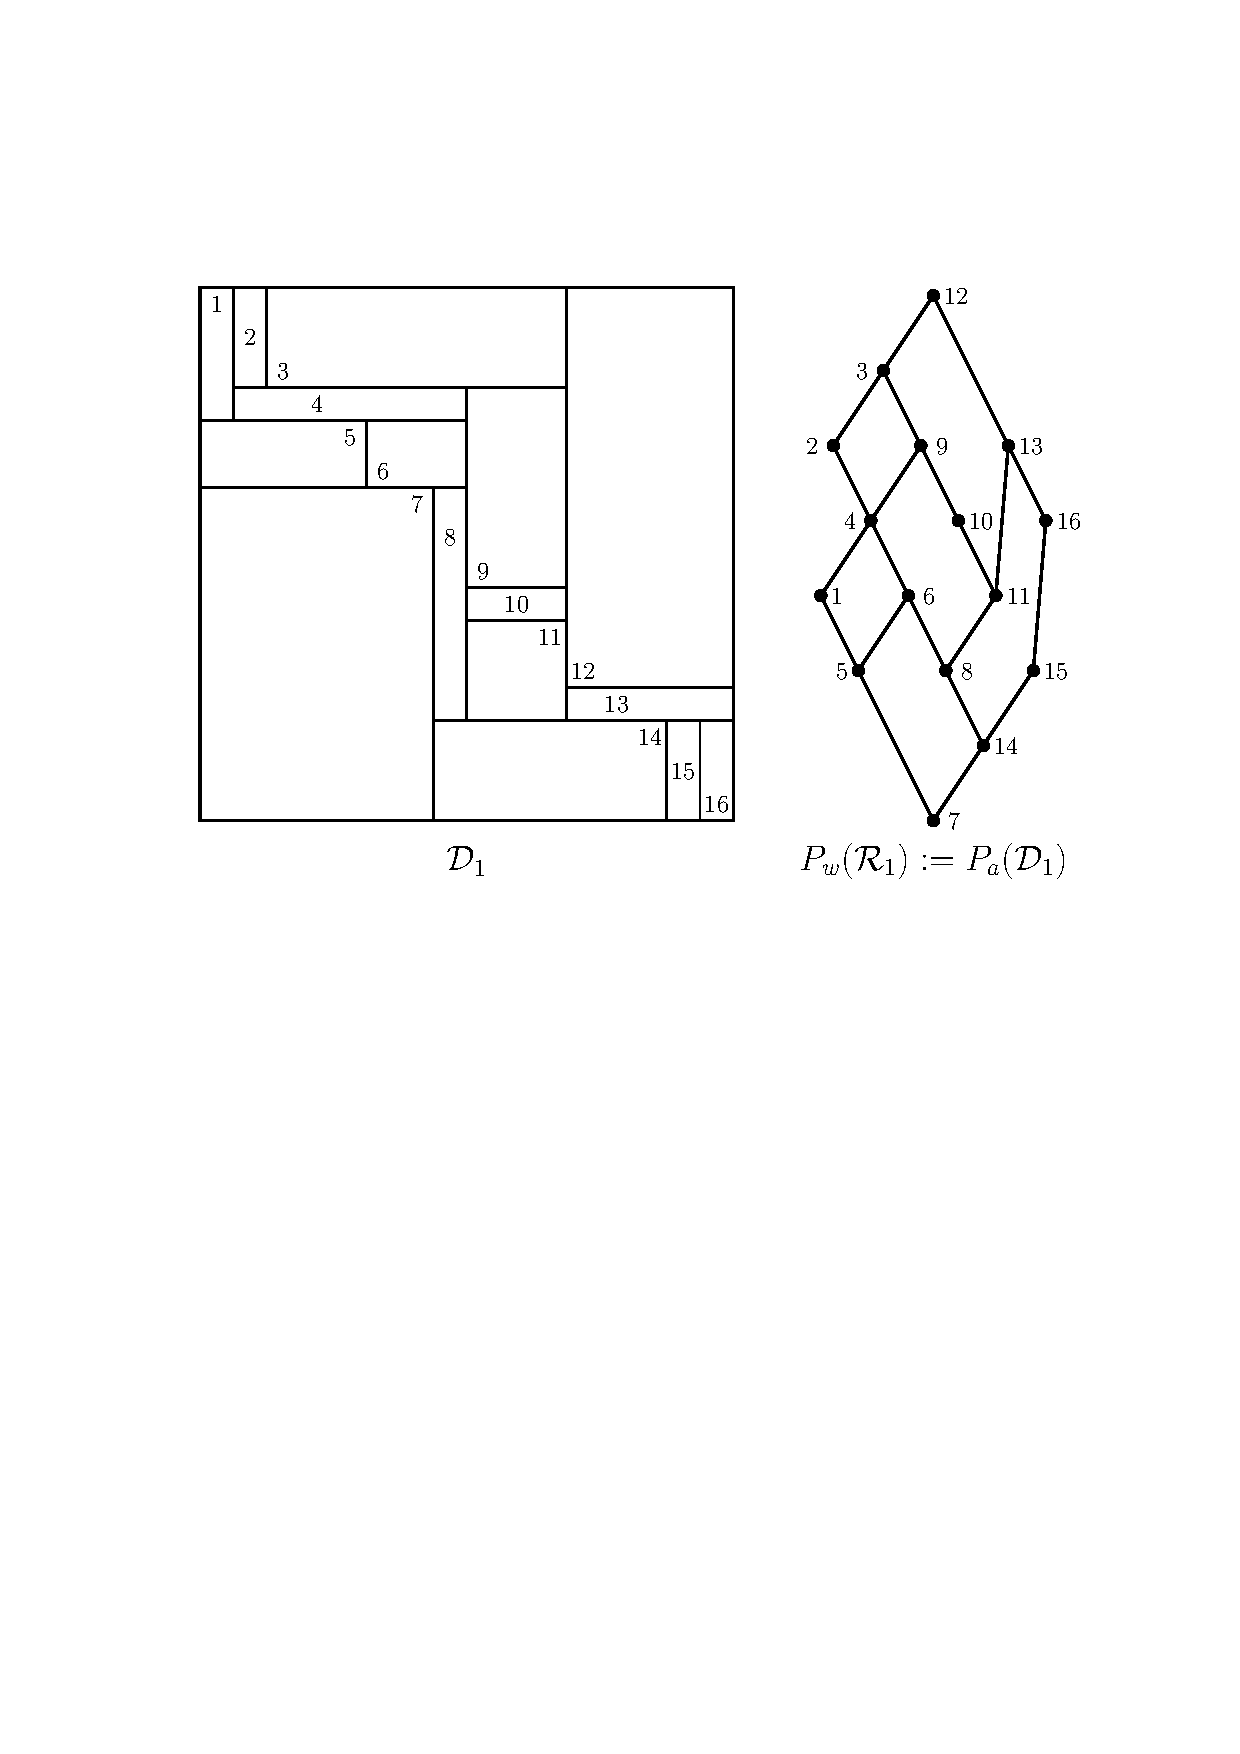
\includegraphics[height=.7\textheight]{w_poset_v2.pdf}
    \end{center}
    \auth{Meehan 2016} 
\end{frame}

\begin{frame}
  \frametitle{The weak rectangulation congruence}
    Linear extensions of adjacency posets.
    \begin{center}
      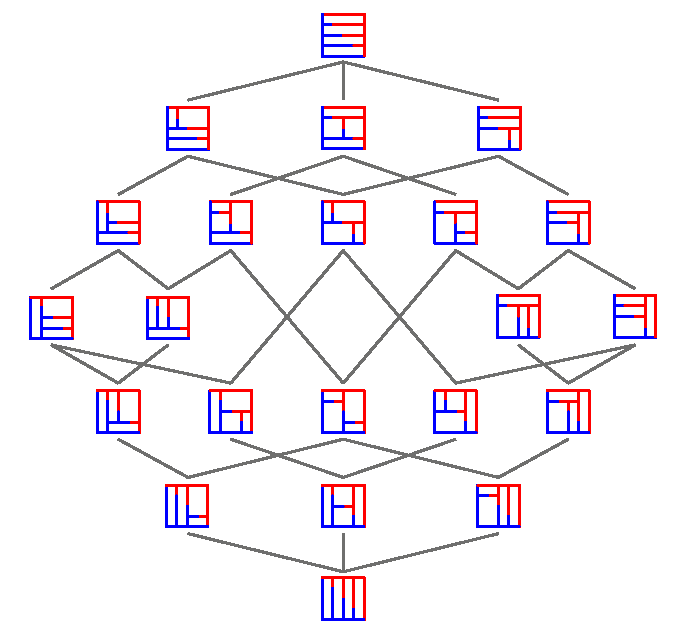
\includegraphics[height=.7\textheight]{weakRectangulationLattice.pdf}
    \end{center}
    \auth{Law-Reading 2010} 
\end{frame}

\begin{frame}
  \frametitle{Weak rectangulotopes}
    \begin{center}
      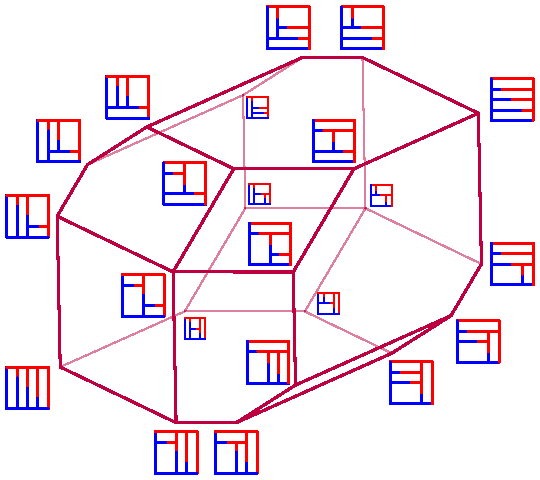
\includegraphics[height=.6\textheight]{weakRectangulotopeLabeled.pdf}
    \end{center}
    \begin{theorem}
      Weak rectangulotopes are Minkowski sums of two opposite associahedra.
      \end{theorem}
    \auth{Law-Reading 2010}
\end{frame}

\begin{frame}
  \frametitle{Loday coordinates for weak rectangulotopes}
  \begin{theorem}
  The weak rectangulotope is realized by the convex hull of the points
  \[
  \sum_{i\in [n]} (\loday{w}^R_i - \antiloday{w}^R_i)\cdot \b{e}_i
  \]
  for all weak rectangulations $R$ of size~$n$,
  with
  \[
    \loday{w}^R_i \eqdef h^T_i\cdot v^T_i
    \qquad\text{and}\qquad
    \antiloday{w}^R_i \eqdef h^S_i\cdot v^S_i,
  \]
  where~$S$ and~$T$ are the twin binary trees of the rectangulation, and $h^T_i$ and $v^T_i$ denote the number of leaves in the horizontal and vertical subtrees of $i$ in~$T$.
  \end{theorem}
  \auth{Law-Reading 2010, C.-Pilaud 2024}
\end{frame}

%--------------------------
%--- Strong rectangulations
%--------------------------

\begin{frame}
  \frametitle{Strong rectangulations}
  Strong equivalence relation:
    \begin{center}
      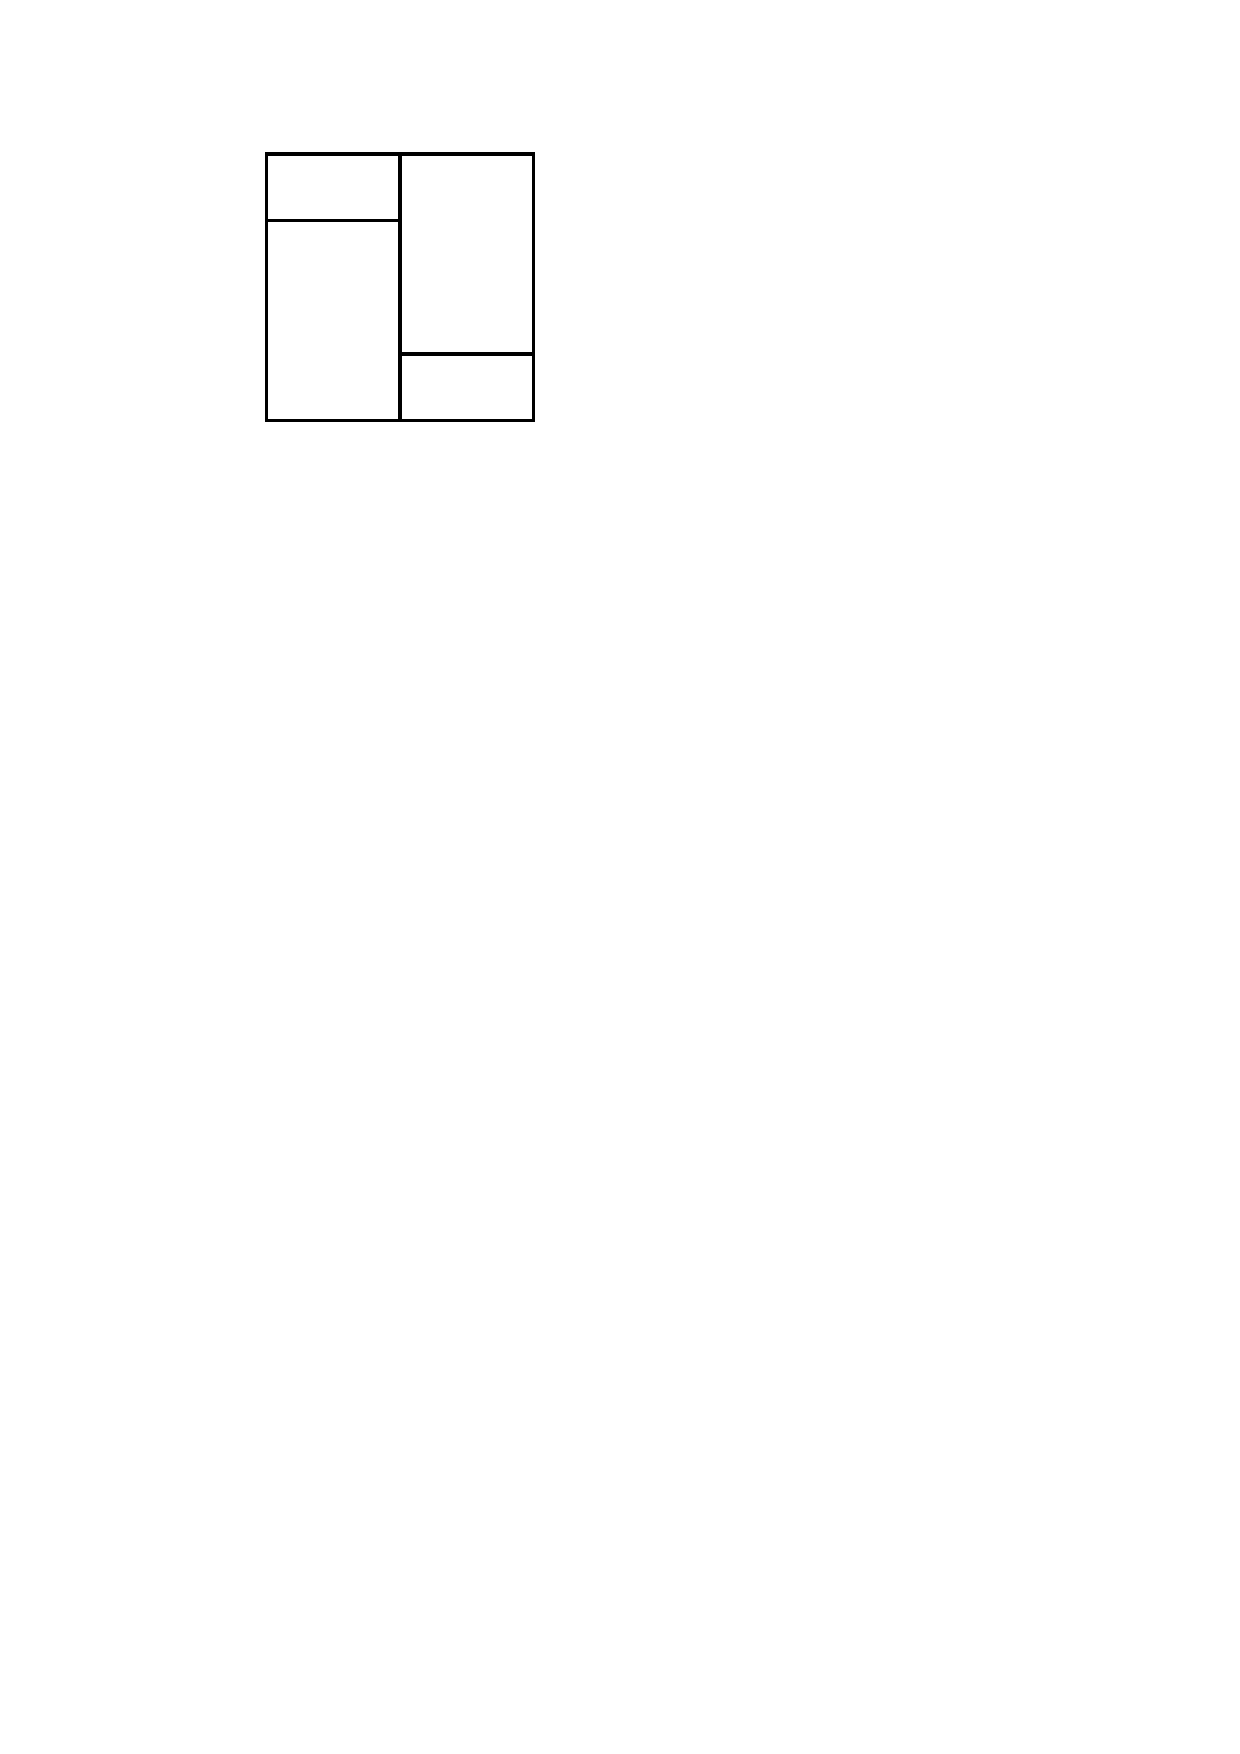
\includegraphics[page=1,height=.1\textheight]{figures.pdf} $\not\equiv$ 
      \includegraphics[page=2,height=.1\textheight]{figures.pdf}
    \end{center}   
    \begin{center}
      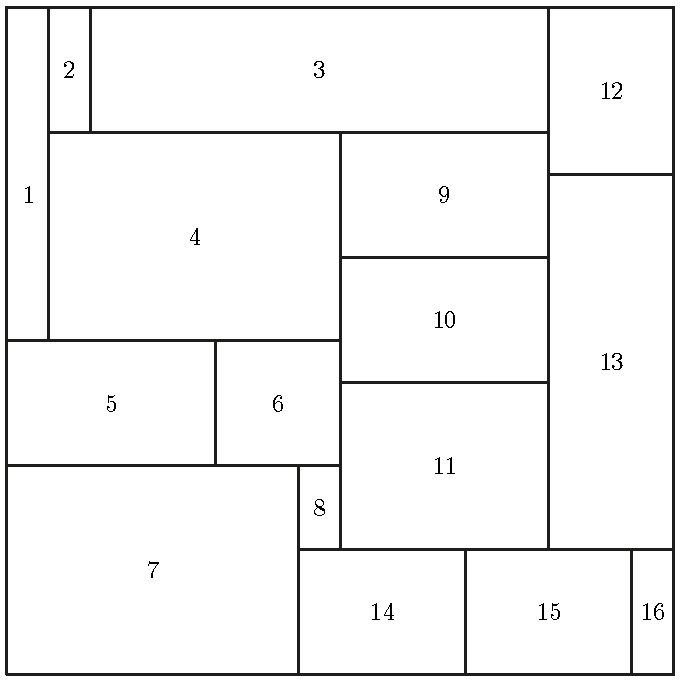
\includegraphics[height=.4\textheight]{strongRectangulation.pdf} $\not\equiv$ 
      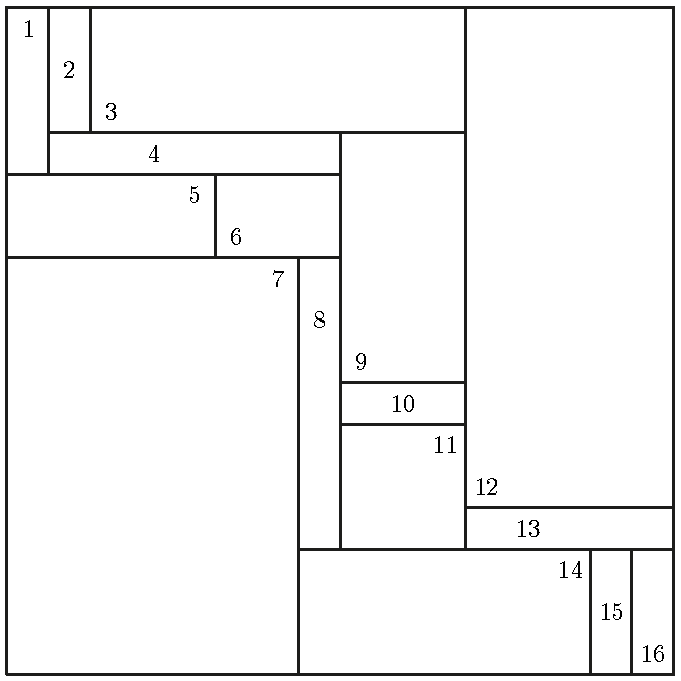
\includegraphics[height=.4\textheight]{weakRectangulation.pdf}
    \end{center}  

  \pause
  \begin{description}
  \item[Bijective] {\em 2-clumped permutations} -- forbidding the patterns 3{\green 51}24, 3{\green 51}42, 24{\green 51}3, and 42{\green 51}3

    \auth{Reading 2012}
    \pause
  \item[Order-theoretic] strong rectangulation lattice
  \item[Polyhedral] strong rectangulotopes
  \end{description}
\end{frame}

\begin{comment}
\begin{frame}
  \frametitle{A surjective map from permutations to rectangulations}
  \[
  \gamma_s : S_n \mapsto \mathcal{SR}_n
  \]
    \begin{center}
  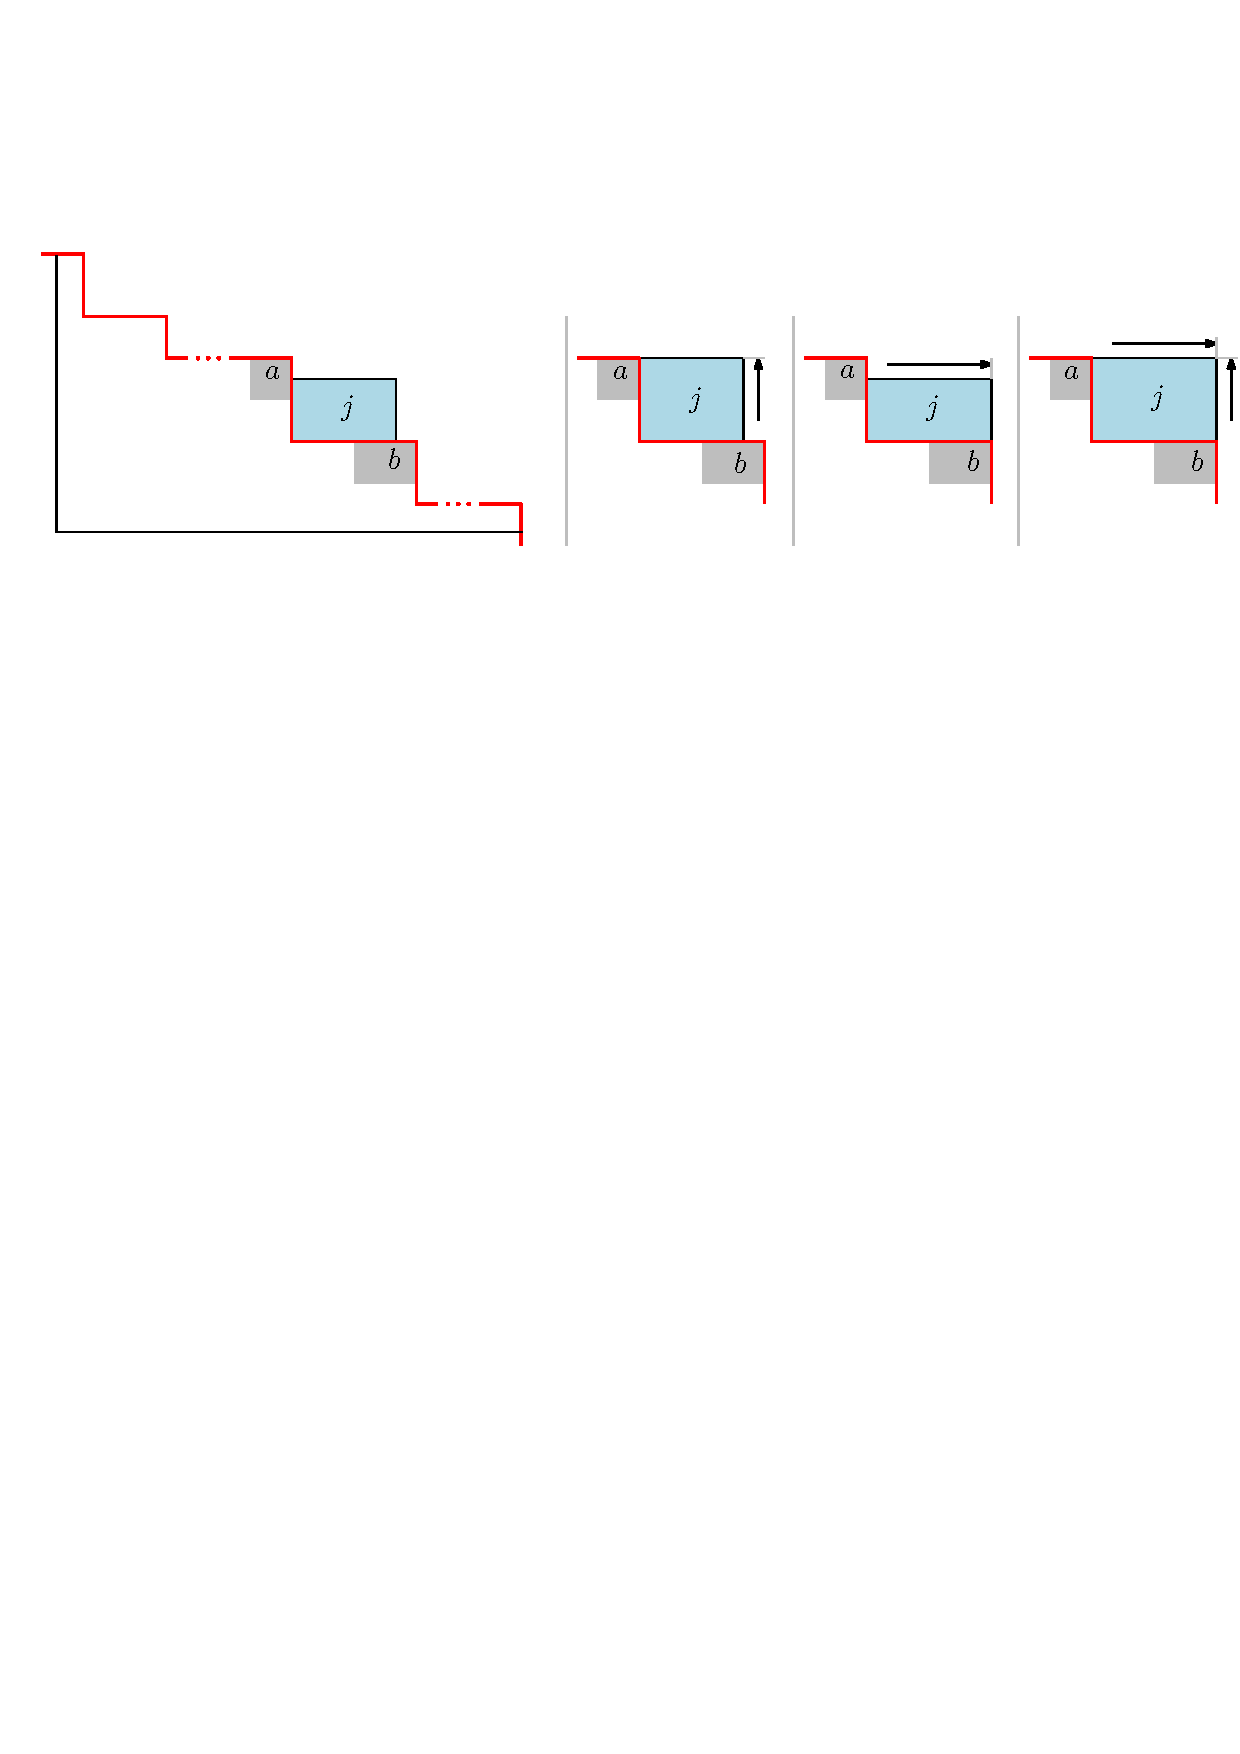
\includegraphics[width=\textwidth]{strong-forward.pdf}
    \end{center}
    \auth{Asinowski, C., Felsner, Fusy 2024}
\end{frame}

\begin{frame}
%  \frametitle{A surjective map from permutations to rectangulations}
  
  \begin{center}
  \includegraphics[page=13,height=\textheight]{Example16.pdf}
  \end{center}
\end{frame}
\end{comment}

\begin{frame}
  \frametitle{Strong poset}
  Adjacency, and two ``special relations'':
  \begin{center}
    \includegraphics[page=4, height=.2\textheight]{strong_poset.pdf}
    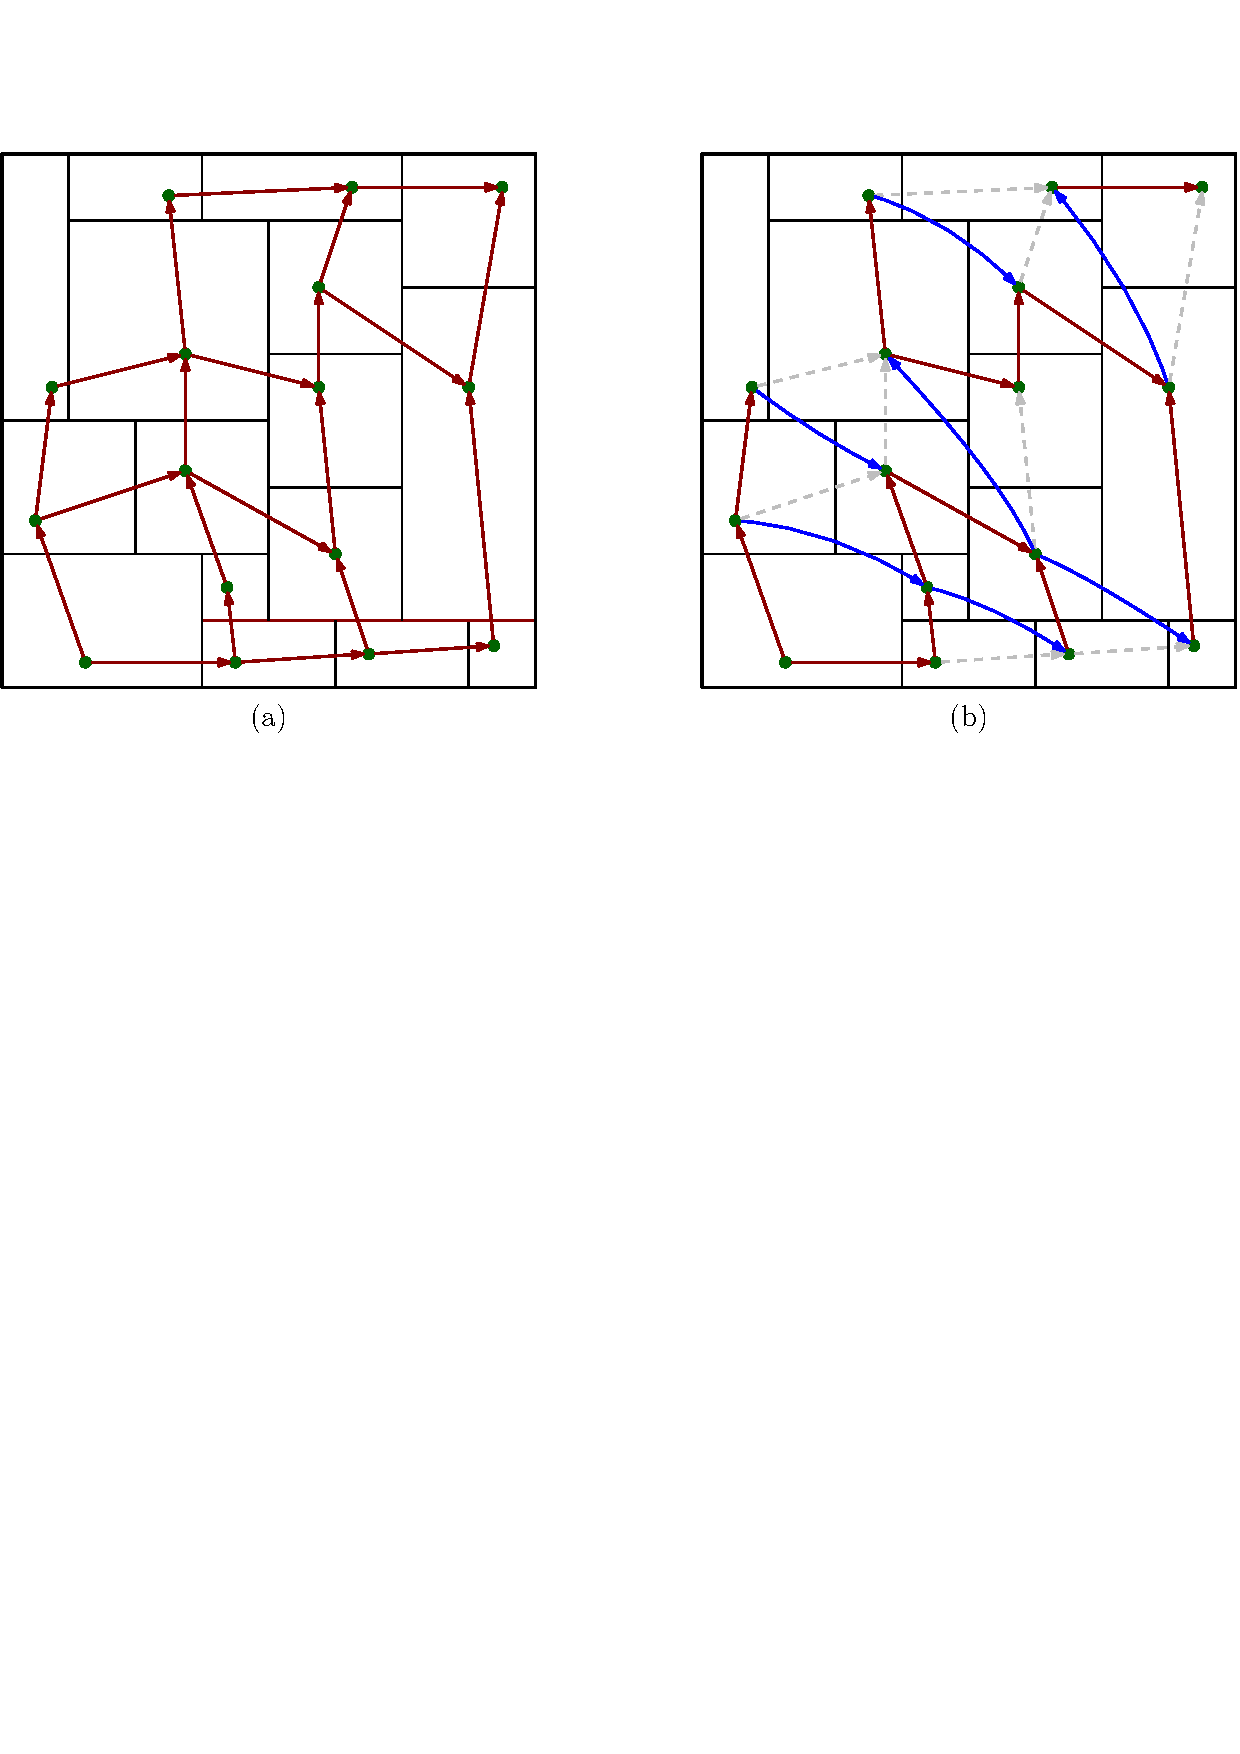
\includegraphics[height=.5\textheight]{s_poset_rect_v1.pdf}
  \end{center}
      \auth{Asinowski, C., Felsner, Fusy 2024}

\end{frame}

\begin{frame}
  \frametitle{The strong rectangulation congruence}
    Linear extensions of strong posets.

    \begin{center}
    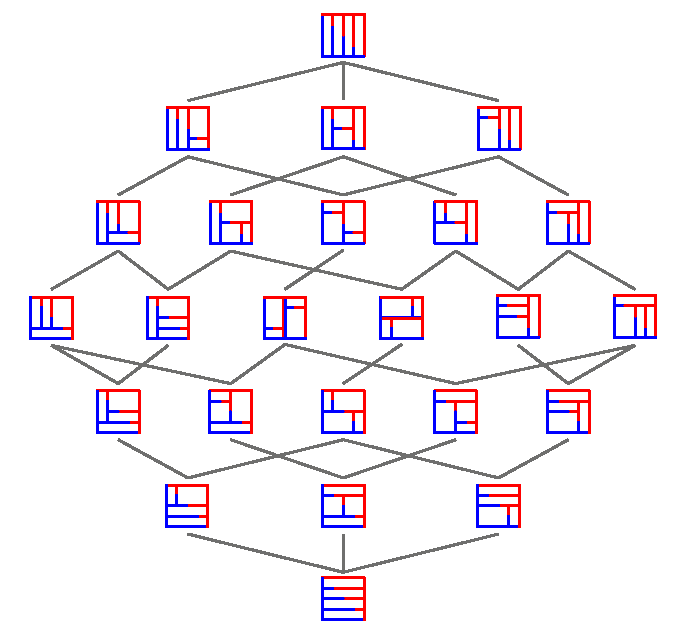
\includegraphics[height=.7\textheight]{strongRectangulationLattice.pdf}
  \end{center}
  \auth{Reading 2012, Asinowski, C., Felsner, Fusy 2024}
\end{frame}

\begin{frame}
  \frametitle{Strong rectangulotopes}
  \begin{center}
    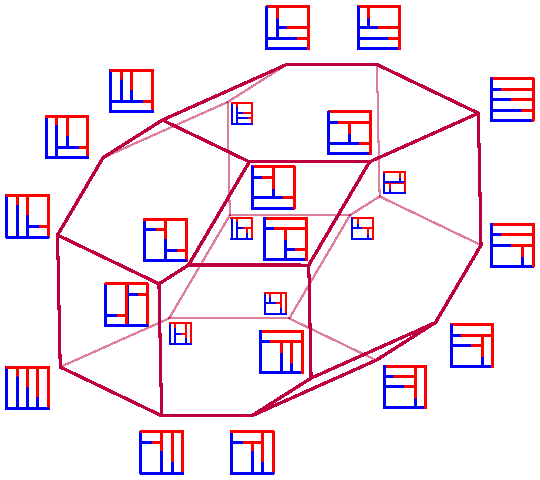
\includegraphics[height=.7\textheight]{strongRectangulotopeLabeled.pdf}
  \end{center}
  Exist thanks to \auth{Pilaud-Santos 2019}
\end{frame}

\begin{frame}
  \frametitle{Flip graph}
  \begin{center}
    \includegraphics[page=2, height=.8\textheight]{gamma-forward.pdf}
  \end{center}
  \auth{Meehan 2019}
\end{frame}

\begin{frame}
  \frametitle{Congruences and arc diagrams}
    \begin{theorem}
    Congruences $\equiv$ of the weak order are one-to-one with {\em arc ideals} $\mathcal{A}_{\equiv}$.
  \end{theorem}
  \auth{Reading 2015}
 \begin{center}
    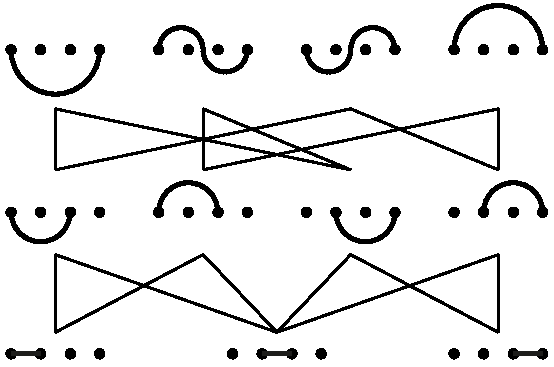
\includegraphics[height=.5\textheight]{subarcOrder.pdf}
  \end{center}
 
\end{frame}

\begin{frame}
  \frametitle{Shard polytopes}
  \begin{theorem}
    The quotientope of a congruence $\equiv$ is the Minkowski sum of the {\em shard polytope} of each arc in $\mathcal{A}_{\equiv}$.
  \end{theorem}
  \auth{Padrol, Pilaud, Ritter 2023}
  \begin{center}
    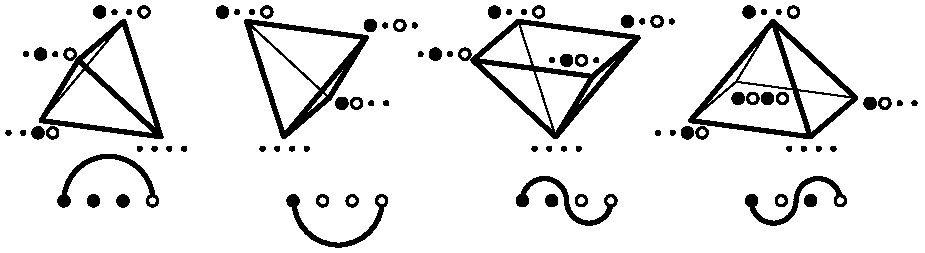
\includegraphics[width=\textwidth]{shardPolytopes.pdf}
  \end{center}
\end{frame}

\begin{frame}
  \frametitle{Intertwined binary trees}
  \begin{center}
    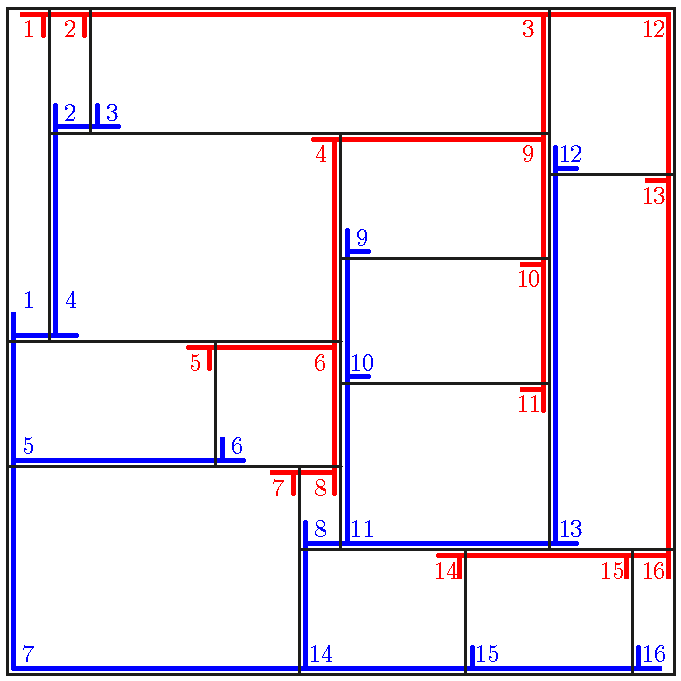
\includegraphics[height=.7\textheight]{strongRectangulationTrees.pdf}
  \end{center}
  \auth{C.-Pilaud 2024}
\end{frame}

\begin{frame}
  \frametitle{Loday coordinates for strong rectangulotopes}

  \begin{theorem}
  The $(n-1)$-dimensional strong rectangulotope is realized by the convex hull of the points
  \[
  \sum_{i< j} (\yin{w}^R_{i,j} - \yang{w}^R_{i,j})\cdot (\b{e}_i - \b{e}_j),
  \]
   for all strong rectangulations $R$ of size~$n$, with
  \[
    \yin{w}^R_{i,j} \eqdef h^T_i \cdot cv^{T,S}_{i,j}\cdot h^S_ j\cdot \llbracket \neg \, i \, \backslash \, j \rrbracket
    \qquad\text{and}\qquad
    \yang{w}^R_{i,j} \eqdef v^S_i \cdot ch^{S,T}_{i,j}\cdot v^T_j \cdot \llbracket \neg \, j \, \backslash \, i \rrbracket,
  \]
 where $ch^{T,S}_{i,j}$ (resp.~$cv^{T,S}_{i,j}$) denote the number of {\em common leaves} of the horizontal (resp.~vertical) subtree of $i$ in $T$ and the horizontal (resp.~vertical) subtree of $j$ in $S$,
  \end{theorem}
  \auth{C.-Pilaud 2024}
\end{frame}

%------------------------------
%--- 
%------------------------------
\begin{frame}
  \frametitle{Conclusion}
  \begin{itemize}
  \item Unified descriptions of bijections between equivalence classes of rectangulations and classes of permutations. See ACFF for more bijections.
    \pause
    \item Complete descriptions of two families of polytopes encoding equivalence classes of rectangulations, which are natural and inistructive examples of quotientopes. See CP (in preparation) for details.
  \end{itemize}

  \pause
  \centering
             {\Huge Thank you!}\\
             
             \vspace{1cm}
             
              
\end{frame}

\end{document}
